\section{Lecture 12}
\subsection{Lecture Notes - Weakly Coupled Oscillators}
Recall from our work two lectures ago that for the 2-mass 3-springs problem, the eigenfrequencies were determined to be:
\[\omega_1 = \sqrt{\frac{k+2k_{12}}{m}}, \quad \omega_2 = \sqrt{\frac{k}{m}}\]
Now, we make the assumption that $k_{12} \ll k$, i.e. that the middle spring joining the masses is quite weak. In this limit, we can clearly see that $\omega_1 \approx \omega_2$. This generates an interesting physical case; here we can define a "middle frequency" which is the average of the two eigenfrequencies above:
\[\omega_0 = \frac{\omega_1 + \omega_2}{2}\]
We could then rewrite $\omega_1, \omega_2$ in terms of $\omega_0$ and a small parameter $\e$:
\[\omega_1 = \omega_0 + \e\]
\[\omega_2 = \omega_0 - \e\]
The general solution could then be written as:
\[\v{z}(t) = C_1\m{1 \\ -1}\exp(i(\omega_0 + \e)t) + C_2\m{1\\1}\exp(i(\omega_0 - \e)t)\]
We can factor this expression, recognizing common terms:
\[\v{z}(t) = \left(C_1\m{1 \\ -1}\exp(i\e t) + C_2\m{1\\1}\exp(-i\e t)\right)\exp(i\omega_0 t)\]
Now, suppose that $C_1 = C_2 = \frac{A}{2}$ (i.e. the two modes are excited to be the same amplitude). We then have that:
\[\v{z}(t) = \frac{A}{T}\m{\exp(i\e t) + \exp(-i\e t) \\ \exp(-i\e t) - \exp(i \e t)}\exp(i\omega_0 t)\]
Then using Euler's formula:
\[\v{z}(t) = A\m{\cos(\e t) \\ -i\sin(\e t)}\exp(i\omega_0 t)\]
Now taking the real part of this:
\[\Re\v{z}(t) = \v{x}(t) = \m{x_1 \\ x_2} = \m{A\cos(\e t)\cos(\omega_0 t) \\ A\sin(\e t)\sin(\omega_0 t)}\]
This result corresponds to a fast oscillation (e.g. at frequency $\omega_0$) modulated by a slower oscillation (at frequency $\e$ which is small by assumption). When graphed, this looks like:
\begin{center}
    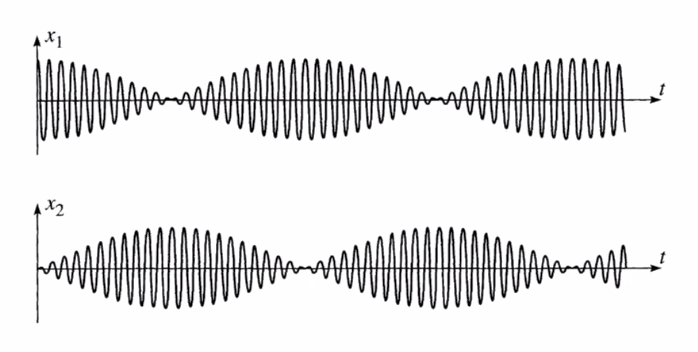
\includegraphics[scale=0.5]{Lecture-12/l12-img1.png}
\end{center}
Where we see "beats"! Exactly like with AM radio waves, we see the frequency stay constant but the amplitude going up and down with time.